%
% klassifikation.tex
% 
% (c) 2019 Prof Dr Andreas Mueller
%
\rhead{Domains}
\section{Domains\label{klassifikation:gebiete}}
\label{domain}
\begin{figure}
\centering
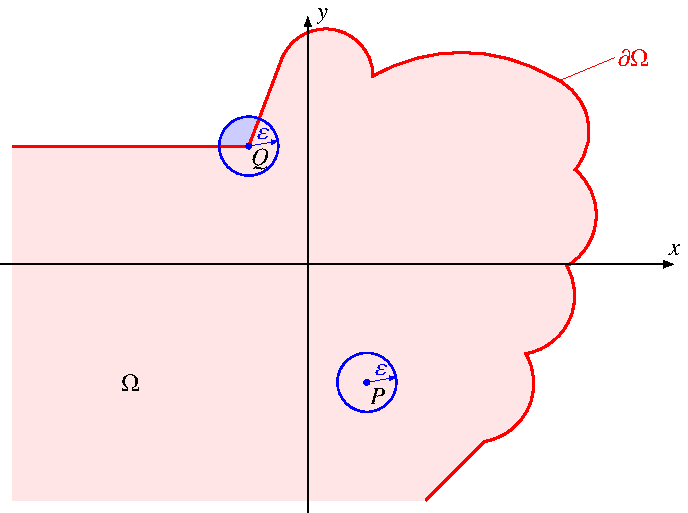
\includegraphics{2-classification/images/domain.pdf}
\caption{Interior points and boundary points of a domain.
The point $P$ is an interior point of $\Omega$ because there is a
small radius $\varepsilon$ such that the ball with radius $\varepsilon$
centered in $P$ is contained in $\Omega$.
The point $Q$ is on the boundary because however small the radius
$\varepsilon$ is chosen, the ball centered in $Q$ always contains some
points in $\Omega$ and some points outside of $\Omega$.
\label{domain:figure}}
\end{figure}
In the theory of ordinary differential equations, we always look for a function
of a single variable, the domain of definition is always an interval.
A solution is fixed by values and derivatives at the endpoints of the interval.

For partial differential equations, the potential domains become much
more interesting.
Just about any subset of $\mathbb R^n$ can be used as the domain of
definition for a differential equation.
The distinction between initial value problems and boundary value
problems that was easy for ordinary differential equations becomes
essentially meaningless.
It turns into the much more difficult question on which parts of
the boundary of the domain we have to prescribe values or derivatives
in order to fix the solution.

The partial derivatives of a function $u$ in a point $(x_1,\dots,x_n)$
are only well defined if the function can be evaluated in a small 
neighborhood of the point.
The derivative is the limit
\[
\frac{\partial u}{\partial x_i}=
\lim_{\Delta x_i\to 0}\frac{u(x_1,\dots,x_i+\Delta x_i, \dots ,x_n)-u(x_1,\dots,x_n)}{\Delta x_i}
\]
where $\Delta x$ is any small vector.
This implies that the differential equation only makes sense in a
domain of definition that contains a small ball around every point
(see figure~\ref{domain:figure}).

\begin{definition}
\label{definition:domain}
A {\em domain}
$\Omega\subset \mathbb R^n$ is an {\em open} subset of
$\mathbb R^n$, i.~e.~every point 
$(x_1,\dots,x_n)\in\Omega$
has a small ball
\[
B(x, r)=\{x'\in\mathbb R^n\,|\,|x-x'|<r\}.
\]
around it that is also contained in $\Omega$, provided $r$ is chosen
small enough but $r>0$:
$B(x,r)\subset\Omega$.
\end{definition}

\begin{beispiel}
The set
\[
\Omega_1=\{ (x,y)\in\mathbb R^2\,|\, 0 < x < 1, 0<y<1\}
\]
is a unit square in the plane without the boundary.
Any point in $\Omega_1$ has a certain minimal distance $r$ to each
boundary of the square.
As a consequence, the disk 
$B(x,r)\subset\Omega_1$ with radius $r$ is still contained in $\Omega_1$.
This means that $\Omega_1$ is open and thus a domain.
\end{beispiel}

\begin{beispiel}
The set
\[
\Omega_2 = \{ (x,y)\in\mathbb R^2\,|\, x\ge 0\}.
\]
is the right half plane including the $y$-axis.
A point on the $y$-axis does not have the property specified in the
definition.
Any small disk around a point on the $y$-axis contains points with negative
$x$-coordinates.
These points do not belong to $\Omega_2$, so no such small disk can be
contained in $\Omega_2$.
Thus $\Omega_2$ is not open and is therefore not a domain.
\end{beispiel}

The difference between the two sets $\Omega_1$ and $\Omega_2$ is
obviously that $\Omega_2$ contains part of the boundary too.

\begin{definition}
\label{definition:boundary}
The {\em boundary} $\partial M$ of a set $M\subset\mathbb R^n$
consists of the points with the property that
any ball around such a point contains points of the set and of its
complement.
\end{definition}
\index{boundary}

There are no boundary points of $\Omega_1$ contained in $\Omega_1$
but all boundary points of $\Omega_2$ are also in $\Omega_2$.
Domains are sets that do not contain any of their boundary points.

\begin{beispiel}
\[
\partial \Omega_1=\emptyset,\qquad\partial \Omega_2=\{(0,y)\,|y\in\mathbb R\}.
\]
\end{beispiel}

\begin{definition}
\label{definition:interior}
If $M\subset\mathbb R^n$ is any subset of $\mathbb R^n$,
then $\mathring M$ denotes the {\em interior} of $M$, the set of all interior
\index{interior}
points, i.~e.~the points with the property that also a small neighborhood
is contained in $M$.
The set of all boundary points is written $\partial M$ and $\bar M$
is the closure is $\bar M=M\cup \partial M$.
\end{definition}

